Our third example is a model of a networked cooperative platoon of
vehicles, which is presented as a benchmark in the ARCH
workshop~\cite{makhlouf2014networked}.  The platoon consists of three
vehicles $M_1$, $M_2$ and $M_3$ along with a leader board ahead $M_4$.
The movement of the vehicles is dependent on the communication between
them their relative distances, velocities and accelerations.  The
distance between a vehicle $M_i$ and its next
vechicle $M_{i+1}$, relative to a reference distances $d_i^{ref}$ is
denoted $e_i$.  The acceleration of the leader vehicle is $a_L$ which
ranges between $[-9,1]m/s$.  The state of the system is denoted
by a vector
$x=\lt[e_1,\dot{e}_1,\ddot{e}_1,e_2,\dot{e}_2,\ddot{e}_2,e_3,\dot{e}_3,\ddot{e}_3\rt]$.
The dynamics of the platoon is different in the two cases when there
is full communication and when there is total failure of
communication.  These dynamics are described by differential equations,
%
\begin{align*}
& \dot{x}=A_cx+B_ca_L~\text{when there is communication}\\
& \dot{x}=A_nx+B_na_L~\text{when there is failure of communication}.
\end{align*}
%
where the pairs of matrices $(A_c,B_c)$ and $(A_n,B_n)$ are different.
The matrices are given in the appendix.  In any given mode, the
dynamics of the system is exponentially stable.  So, the lyapunov
exponent (measure of stability) is higher in case of slow switching
than fast switching.  Therefore, in our evaluation of this example, we
also consider a model having integer switching times, which is less
stable.

%
\begin{table}
\caption{Matices for discrete time slow switching model}~\label{matrices:slow}
{\scriptsize
$A_1=\mymatrix{0.2766  &  0.2855&   -0.0235&    0.2550&    0.2352&   -0.0429&    0.1245&    0.0956&   -0.0234\\
   -0.0917&   -0.0848&    0.0392&   -0.0517&    0.0134&    0.0023&    0.0003&    0.0385 &  -0.0166\\
   -0.0531&   -0.0485&    0.0404&    0.0434&    0.0807&   -0.0172&    0.0301&    0.0363&   -0.0097\\
    0.1406&    0.1632&    0.0002&    0.0313&    0.1166&   -0.0122&    0.1017&    0.1309&   -0.0431\\
   -0.0411&   -0.0589&   -0.0421&   -0.0512&   -0.1530&    0.0575&   -0.0476&   -0.0321&    0.0051\\
   -0.0393&   -0.0402&   -0.0111&   -0.0641&   -0.0754&    0.0467&    0.0497&    0.0760&   -0.0251\\
    0.0628&    0.0763&    0.0095&    0.0634&    0.0987&    0.0081&   -0.0788&    0.0489&   -0.0436\\
   -0.0088&   -0.0158&   -0.0081&   -0.0351&   -0.0452&   -0.0726&   -0.0621&   -0.2082&    0.0863\\
   -0.0246&   -0.0235&   -0.0078&   -0.0572&   -0.0547&   -0.0183&   -0.1049&   -0.1146&    0.0307}$
$A_2=\mymatrix{ 0.2398 &   0.2204&   -0.0715&   -0.0000&    0.0000&   -0.0000&   -0.0000&    0.0000&   -0.0000\\
   -0.1148&   -0.1083&    0.0352&   -0.0000&   -0.0000&    0.0000&   -0.0000&   -0.0000&    0.0000\\
   -0.0565&   -0.0567&    0.0176&   -0.0000&   -0.0000&   -0.0000&   -0.0000&   -0.0000&    0.0000\\
    0.0178&    0.5068 &  -0.0658&    0.2410&    0.3042&   -0.1113&   -0.0000&    0.0000&   -0.0000\\
   -0.1056&  -0.3026&    0.0327&   -0.1329&   -0.1627&    0.05657&   -0.0000&   -0.0000&    0.0000\\
   -0.1089&   -0.1100&   -0.0055&   -0.0675&   -0.0720&    0.0204&   -0.0000&   -0.0000&    0.0000\\
    0.2386&   -0.0802&    0.0965&    0.1118&    0.1544&    0.0604&    0.1197&    0.2679&   -0.1103\\
    0.0762&    0.3143&   -0.0998&   -0.0213&   -0.0283&   -0.0726&   -0.1404&   -0.2191&    0.0779\\
   -0.0043&    0.0212&   -0.0122&   -0.0468&   -0.0413&   -0.0171&   -0.0991&   -0.0990&    0.0251}$
 $B_1=\mymatrix{1.8593\\
    0.2855\\
    1.0848\\
    0.5394\\
    0.1632\\
    1.1437\\
    0.1950\\
    0.0763\\
    1.1596}$
$B_2=\mymatrix{1.7651\\
    0.2204\\
    1.1083\\
    2.1977\\
    0.5068\\
    1.4109\\
   -1.2748\\
   -0.0802\\
    1.0966}$
$B_3=\mymatrix{2.8411\\
    0.0019\\
    1.0006\\
    0.9508\\
    0.0007\\
    1.0009\\
    0.3775\\
    0.0003\\
    1.0009}$    
$B_4=\mymatrix{2.2276\\
    0.0001\\
    1.0001\\
    2.7152\\
   -0.0005\\
    1.0000\\
   -0.4469\\
    0.0001\\
    1.0000\\
}$
~~$A_3=A_4=\repmat{0}{9}{9}$.
}
\end{table}
%
\begin{table}
\caption{Matrices for discrete time fast switching model}~\label{matrices:fast}
{\scriptsize
$A_1=A_3=\mymatrix{ 0.8902 &   0.6370&   -0.1484&    0.0588&   -0.0050&    0.0001&    0.0157&   -0.0148&    0.0059\\
   -0.2340&    0.1889&   -0.1119&    0.1267&    0.0147&   -0.0039&    0.0363&   -0.0201&    0.0104\\
    0.1755&    0.7560&   -0.2251&   -0.0959&   -0.0989&    0.0181&   -0.0373&   -0.0273&    0.0018\\
    0.0462&    0.0643&    0.1514&    0.8509&    0.7076&   -0.1685&    0.0303&    0.0218&   -0.0038\\
    0.0934&    0.1271&    0.1151&   -0.3284&    0.2923&   -0.1466&    0.0660&    0.0517&   -0.0108\\
    0.1262&    0.6998&    0.0092&    0.1826&    0.7469&   -0.2119&   -0.0885&   -0.0830&    0.0189\\
    0.0116&    0.0170&    0.0026&    0.0241&    0.0282&    0.1719&    0.8532&    0.7238&   -0.1801\\
    0.0256&    0.0364&    0.0064&    0.0505&    0.0619&    0.1543&   -0.3320&    0.3231&   -0.1730\\
    0.1047&    0.6724&    0.0017&    0.1502&    0.6976&    0.0119&    0.2247&    0.7581&   -0.1875}$
$A_2=A_4=\mymatrix{0.8898 &   0.6325&   -0.1463&    0.0000&    0.0000&    0.0000&    0.0000&    0.0000&   -0.0000\\
   -0.2348&    0.1775&   -0.1094&    0.0000&    0.0000&    0.0000&    0.0000&    0.0000&   -0.0000\\
    0.1756&    0.7674&   -0.2136&    0.0000&    0.0000&    0.0000&    0.0000&    0.0000&   -0.0000\\
    0.0939&    0.3146&    0.1064&    0.9098&    0.6995&   -0.1686&    0.0000&    0.0000&   -0.0000\\
    0.1708&    0.6120&    0.0043&   -0.2012&    0.2985&   -0.1533&    0.0000&    0.0000&   -0.0000\\
    0.1687&    0.5757&    0.1151&    0.1829&    0.7569&   -0.1980&    0.0000&    0.0000&   -0.0000\\
   -0.0364&   -0.2331&    0.0460&    0.0254&    0.0312&    0.1721&    0.9004&    0.7304&   -0.1778\\
   -0.0529&   -0.4476&    0.1169&    0.0548&    0.0704&    0.1571&   -0.2263&    0.3541&   -0.1728\\
    0.1044&    0.6771&   -0.0016&    0.1418&    0.6953&    0.0121&    0.2199&    0.7571&   -0.1877}$    
$B_1=B_3=\mymatrix{0.3930\\
    0.6370\\
    0.8111\\
    0.0200\\
    0.0643\\
    0.6840\\
    0.0051\\
    0.0170\\
    0.6476\\
}$
$B_2=B_4=\mymatrix{0.3918\\
    0.6325\\
    0.8225\\
    0.0979\\
    0.3146\\
    0.2105\\
   -0.0727\\
   -0.2331\\
    0.6581}$
}
\end{table}
%
%
\begin{figure}
\center
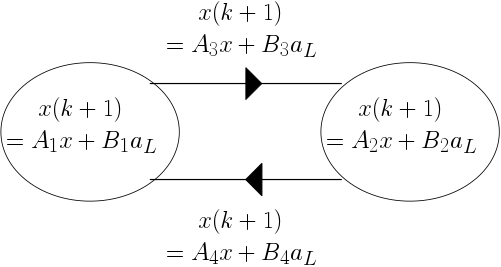
\includegraphics[scale=0.5]{fig/platton-dynamics.png}
\caption{Time discretized model of networked platoon}~\label{fig:model-platoon}
\end{figure}
%

\begin{table}
\begin{tabular}{|l|c|c|c|c|c|}
\hline
\multicolumn{2}{|c|}{\multirow{4}{*}{Method}} & \multicolumn{4}{|c|}{\multirow{2}{*}{Slow switching}}\\
\multicolumn{2}{|c|}{} & \multicolumn{4}{|c|}{}\\
\cline{3-6}
\multicolumn{2}{|c|}{} & \multirow{2}{*}{$-e_1\leq$} & \multirow{2}{*}{$-e_2\leq$} & \multirow{2}{*}{$-e_3\leq$} & Comp.\\
\multicolumn{2}{|c|}{} & & & & time (s)\\
\hline
\multirow{4}{*}{SpaceEx} & octagon & \multirow{2}{*}{28} &
\multirow{2}{*}{27} & \multirow{2}{*}{10}& \multirow{2}{*}{$>180s$}\\
& template & & & &\\
\cline{2-6}
& 100 support & \multirow{2}{*}{28} & \multirow{2}{*}{25} &
\multirow{2}{*}{13} & \multirow{2}{*}{1.3}\\
& vectors & & & &\\
\hline
\multicolumn{2}{|c|}{\multirow{2}{*}{Real zonotope~\cite{makhlouf2014networked}}} &
\multirow{2}{*}{25} & \multirow{2}{*}{25} & \multirow{2}{*}{10} & \multirow{2}{*}{n/a}\\
\multicolumn{2}{|c|}{} & & & &\\
\hline
\multicolumn{2}{|c|}{\multirow{2}{*}{Augmented complex zonotope}} &
\multirow{2}{*}{28} & \multirow{2}{*}{26} &
\multirow{2}{*}{12} & \multirow{2}{*}{12}\\
\multicolumn{2}{|c|}{} & & & & \\
\hline
\end{tabular}
\caption{Expermimental results: Slow switching networked platoon}~\label{tab:largedwell-platoon}
%
\end{table}

\begin{table}
\begin{tabular}{|l|c|c|c|c|c|}
\hline
\multicolumn{2}{|c|}{\multirow{4}{*}{Method}} & \multicolumn{4}{|c|}{\multirow{2}{*}{Fast switching}}\\
\multicolumn{2}{|c|}{} & \multicolumn{4}{|c|}{}\\
\cline{3-6}
\multicolumn{2}{|c|}{} & \multirow{2}{*}{$-e_1\leq$} & \multirow{2}{*}{$-e_2\leq$} & \multirow{2}{*}{$-e_3\leq$} & Comp.\\
\multicolumn{2}{|c|}{} & & & & time (s)\\
\hline
\multirow{4}{*}{SpaceEx} & octagon & \multirow{2}{*}{$>1000$} &
\multirow{2}{*}{$>1000$} & \multirow{2}{*}{$>1000$} &
\multirow{2}{*}{$>180s$}\\
& template & & & &\\
\cline{2-6}
& 100 support & \multirow{2}{*}{$>1000$} & \multirow{2}{*}{$>1000$} &
\multirow{2}{*}{$>1000$} & \multirow{2}{*}{$>180s$}\\
& vectors & & & & \\
\hline
\multicolumn{2}{|c|}{\multirow{2}{*}{Augmented complex zonotope}} &
\multirow{2}{*}{46} & \multirow{2}{*}{54} &
\multirow{2}{*}{57} & \multirow{2}{*}{12.6}\\
\multicolumn{2}{|c|}{} & & & & \\
\hline
\end{tabular}
%
\caption{Expermimental results: Fast switching networked Platoon}~\label{tab:largedwell-platoon1}
\end{table}

{\bf Time discretized models: } We could discretized the dynamics of
both models with large minimum switching time and integer switching
time.  The time discretized model has 2 locations and 4 edges, as
described in Figure~\ref{fig:model-platoon}.  The continuous state is
9-dimensional.  The matrices denoted in the figure are different for
the case of slow switching and fast switching and are given in
Tables~\ref{matrices:slow} and~\ref{matrices:fast}, respectively.


{\bf Linear invariance property: } The verification challege proposed
in~\cite{makhlouf2014networked} is to find the minimum possible reference distances
$d_i^{ref}~\forall i\in\set{1,2,3}$, such that the vehicles do not
collide.  Any set of upper bounds on $-e_1$, $-e_2$, and $-e_3$ are
safe lower limits on the respective reference distances.  We express
the verification challege in terms of linear invariance properties, we
follows.  For each ${T_i:~1\leq
i\leq 3}$, where
%
$ T_1=\mymatrix{-1 & \repmat{0}{1}{8}},~
T_2=\mymatrix{\repmat{0}{1}{3} & -1 &\repmat{0}{5}{3}}$ and
 ${T_3=\mymatrix{\repmat{0}{1}{6}& -1 &\repmat{0}{2}{3}}},
$
%
find an upper bound on each $d_i:~i\in\set{1,2,3}$ such that
$\lt(T_i,d_i\rt)$ is a linear invariance property of the system.

\tbf{Experiment settings.}  We chose the primary template
as the collection of the (complex) eigenvectors of linear matrices of
the affine maps in the the two locations and their binary products,
the axis aligned box template and the templates used for
overapproximating the input sets. For the SpaceEx tool, we
experimented with two templates, octagon and hundred uniformly sampled
support vectors.

\tbf{Results.}  For the large minimum dwell time of $20s$, the
discrete time SpaceEx implementation and also a method based on using
real zonotopes~\cite{makhlouf2014networked} could verify slightly
smaller bounds compared to our approach.  But for the small minimum
dwell time ($1s$) model, SpaceEx could not even find a finite set of
bounds, whereas our approach could verify a finite set of bounds.  The
reason is that the fast system model is more stable compared to the
slow switching.  Possibly because complex zonotope captures
contraction along complex eigenvectors, we could find a finite
invariant for even the less stable fast switching model.  These
results are reported in the Tables~\ref{tab:largedwell-platoon}
and~\ref{tab:largedwell-platoon1}.
%
